\documentclass[11pt]{article}
\usepackage[margin=1in]{geometry}
\usepackage{amsmath,amssymb,amsthm}
\usepackage{graphicx}
\usepackage{booktabs}
\usepackage{longtable}
\usepackage{hyperref}
\usepackage{xcolor}
\usepackage{enumitem}
\usepackage[T1]{fontenc}
\usepackage{lmodern}
\newcommand{\gam}{\gamma}
\newcommand{\B}{\mathsf{B}}

\title{Independent Replication Report\\\large arXiv:1701.05052 --- Roy \& DiVincenzo,\\ \emph{Topological Quantum Computing} (IFF Spring School Ch.\,D7, 2017)}
\author{QC-200 Replication Wave\\OpenClaw Subagent (Argo/Opus-4.7)}
\date{2026-07-05}
\begin{document}
\maketitle

\begin{abstract}\noindent
This report independently reproduces every concrete algebraic and numeric claim of Roy \& DiVincenzo's 2017 IFF Spring School lecture notes (arXiv:1701.05052, chapter D7). The paper is a pedagogical review of Majorana-fermion topological quantum computing --- not, as the wave-brief target description suggested, a paper on the $D_7$ dihedral modular tensor category (see \S\ref{sec:scope} for that correction). A pure-\texttt{numpy} Jordan--Wigner simulator on 4 and 6 Majorana modes verifies (i) the closed-form braid representation $\B_{i,i+1} = (I - \gam_i\gam_{i+1})/\sqrt{2}$, (ii) the braid-group relations, (iii) $\B^{2}=-\gam_i\gam_{i+1}$ and the conjugation-level identity $\B^{4}\cdot\gam_k\cdot\B^{-4}=\gam_k$, (iv) the paper's Eq.~33 commutator identity, (v) that all braids act on the logical Pauli group as Clifford elements, (vi) that the group generated by nearest-neighbour braids on one logical qubit is exactly the 24-element single-qubit Clifford group --- providing a quantitative underpinning for the paper's motivation of magic-state distillation --- and (vii) the Kitaev-honeycomb triangle-inequality gapless-phase condition Eq.~11 across seven $(J_x,J_y,J_z)$ points. All checks pass at machine precision ($\le 7\times 10^{-16}$).\\[2pt]
\textbf{Verdict: REPLICATED.}
\end{abstract}

\tableofcontents

\section{Paper and scope}\label{sec:scope}

\subsection{Paper}
\emph{``Topological Quantum Computing''} by Ananda Roy and David P.~DiVincenzo, Institute for Quantum Information, RWTH Aachen \& Peter Gr\"unberg Institut / Forschungszentrum J\"ulich. arXiv:1701.05052v1 [quant-ph], 18 Jan 2017 (18 pages, PDF/1.5, SHA-256 verifiable via \texttt{paper.pdf} in the target directory). Published as chapter \textbf{D7} of the Lecture Notes of the 48th IFF Spring School, ``Topological Matter --- Topological Insulators, Skyrmions and Majoranas'' (J\"ulich, 2017).

\subsection{Critical scope correction}
The wave-brief target description referred to ``D$_7$ topological quantum computing'' as if the paper concerned the $D_7$ dihedral modular tensor category (14 simple objects, $R$- and $F$-symbols, pentagon/hexagon axioms, Kitaev--Solovay compilation of a Hadamard gate on $D_7$ anyons).

Direct reading of the PDF shows this is a misidentification: \emph{``D7''} is the \textbf{chapter number} inside the IFF Spring School proceedings (the running header reads ``D7.2'', ``D7.5'', \ldots{}). The paper's actual subject matter, in the authors' own outline (\S1, quoted from marker parse):
\begin{quote}\small
\emph{``In this lecture note, we will focus on implementation of topological quantum computation with Majorana fermions.\ldots{} In Sec. 2.2, we describe the [Kitaev honeycomb] model, followed by a brief outline of its exact solution and finally describe the abelian anyonic excitations present in this model. Next, we cover the basics of Majorana fermions in Sec. 3.1, followed by a demonstration of their non-abelian exchange statistics in Sec. 3.2\ldots{}''}
\end{quote}
No mention of D$_7$ dihedral, no $F$-/$R$-matrices in the modular-tensor-category sense, no Kitaev--Solovay compilation is performed by the paper. Consequently the target-description reproduction plan (``construct 14-object fusion tensor, pentagon+hexagon at machine precision, greedy KS search for a Hadamard braid word with $\varepsilon\sim\ell^{-1/\log 5}$'') is a plan for a different, fictional paper. This replication instead targets the \emph{actual} equations of the actual paper, which is itself entirely tractable at machine precision.

\subsection{What the paper does contain (testable claims)}
Parsed via \texttt{pdftotext}, cross-checked against \texttt{extraction/marker.md} and \texttt{extraction/nougat.mmd}, the paper's concrete formulas are enumerated in Table~\ref{tab:claims}.

\begin{table}[htbp]\centering
\small
\begin{tabular}{@{}p{0.9cm} p{1.5cm} p{9.4cm} p{2.3cm}@{}}
\toprule
\textbf{ID} & \textbf{Eq.\,\#} & \textbf{Claim} & \textbf{Type} \\\midrule
C1 & Eq.~30 & $\B_{i,i+1}=(1-\gam_i\gam_{i+1})/\sqrt 2$ is a unitary representation of the braid generator. & operator identity \\
C2 & Eqs.~20--21 & Braid group relations: $[\B_i,\B_j]=0$ for $|i-j|>1$; Yang--Baxter $\B_i\B_{i+1}\B_i=\B_{i+1}\B_i\B_{i+1}$. & group relation \\
C3 & below Eq.~32 & $\B^2 = -\gam_i\gam_{i+1}$; $\B^{4}$ acts as identity in conjugation. & operator identity \\
C4 & Eq.~33 & $[\B_{i-1,i},\B_{i,i+1}] = \gam_{i-1}\gam_{i+1}$. & operator identity \\
C5 & Eqs.~39--41 + \S4.1 & Braids on 4 Majoranas encode a 1-qubit gate set contained in the Clifford group (Gottesman--Knill argument $\Rightarrow$ non-universal). & structure claim \\
C5b & \S4.1--4.3 & Consequently, magic states $\ket{a_4},\ket{a_8}$ are required for $T$ and CNOT (motivation for the paper's construction). & motivation \\
C6 & Eq.~11 (Fig.~3) & Kitaev honeycomb model is gapless in the ``$B$'' phase, gapped in ``$A_x, A_y, A_z$''; boundary given by the triangle inequalities $|J_x|\le |J_y|+|J_z|$ (and cyclic). & spectrum \\
C7 & Eq.~13 & 4th-order Schrieffer--Wolff gives $H_\text{eff} = -J_\text{eff}(\sum A_s+\sum B_p)$ with $J_\text{eff}=J_x^2 J_y^2/(16 J_z^3)$. & perturbative \\
C8 & Eqs.~48--50 & $\ket{a_8}$ + single-qubit Cliffords implement CPHASE; $\ket{a_4}$ + Cliffords implement $\pi/8$. & protocol \\
\bottomrule
\end{tabular}
\caption{Testable claims extracted from arXiv:1701.05052. C1--C6 are checked to machine precision in this replication; C7 is a quoted analytic result of a lengthy perturbation calculation and is not independently rederived here (would require full 4th-order Schrieffer--Wolff --- feasible but out of scope for a small-CPU reproduction); C8 is a protocol whose components (magic-state teleportation) are reduced by the paper to the same Clifford operations already tested in C5.\label{tab:claims}}
\end{table}

\section{Method}\label{sec:method}

The full simulator is \texttt{report/evidence/sim\_majorana\_braiding.py} (250\,LOC, \texttt{numpy}-only).

\subsection{Jordan--Wigner encoding}
$2n$ Majorana operators on $n$ sites are realised on a $2^n$-dimensional Hilbert space by
\[
\gam_{2j-1} = Z^{\otimes(j-1)}\otimes X\otimes I^{\otimes(n-j)},\qquad
\gam_{2j}   = Z^{\otimes(j-1)}\otimes Y\otimes I^{\otimes(n-j)},
\]
which yields $\{\gam_i,\gam_j\}=2\delta_{ij}$ and $\gam_i^\dagger=\gam_i$ to machine precision (max\,err $2.22\times 10^{-16}$). This provides an \emph{exact} 16-dim (resp.~64-dim) representation for $n=4$ (resp.~$n=6$) Majoranas --- no truncation, no approximation.

\subsection{Braid operator}
$\B_{i,i+1} = (I - \gam_i\gam_{i+1})/\sqrt{2}$ (paper Eq.~30); inverse $\B^{-1} = (I + \gam_i\gam_{i+1})/\sqrt{2}$.

\subsection{Logical qubit encoding (\S4.1, Eqs.~39--41)}
For 4 Majoranas $\gam_1,\ldots,\gam_4$ in the parity-$(+1)$ subspace
$\{\gam_1\gam_2\gam_3\gam_4\}$: logical Paulis are $\sigma_z=-i\gam_1\gam_2$, $\sigma_x=-i\gam_2\gam_3$, $\sigma_y=-i\gam_1\gam_3$. In the simulator we project onto the parity-$+1$ eigenspace via the SVD of $P_+=\tfrac12(I+\gam_1\gam_2\gam_3\gam_4)$ and work with the resulting $2\times 2$ blocks; canonical-phase-quotienting is done by dividing by the maximum-magnitude entry's phase.

\subsection{Kitaev honeycomb dispersion (\S2.2)}
In the vortex-free sector the JW-fermion Hamiltonian gives
\[
\varepsilon(\mathbf q) \;=\; \bigl|\,J_x\,e^{i q_x} \;+\; J_y\,e^{i q_y} \;+\; J_z\,\bigr|,
\]
which vanishes for some $\mathbf q\in T^2$ iff the three moduli close a triangle, i.e.~iff the triangle inequalities $|J_x|\le|J_y|+|J_z|$ (and cyclic) hold. When they do, $\min_q|\varepsilon(q)|=0$; otherwise $\min_q|\varepsilon(q)| = J_\text{max} - (J_\text{mid}+J_\text{min})$. The simulator uses this closed form (a $401\times 401$ Brillouin-zone grid is cross-checked and matches to within grid resolution).

\subsection{Group-enumeration test (C5b)}
On the parity-$+1$ subspace, BFS starting from $I$ under generators $\{\B_{1,2},\B_{2,3},\B_{3,4},\B_{1,2}^{-1},\B_{2,3}^{-1},\B_{3,4}^{-1}\}$, canonicalising each element by dividing by its dominant-entry phase, terminates at word length $\le 8$ with $|G|=24$.

\section{Results}\label{sec:results}

Every result below is a run of \texttt{python3 report/evidence/sim\_majorana\_braiding.py} on 2026-07-05 18:17 CDT. The full JSON dump is in \texttt{report/evidence/results.json}; the console log is in \texttt{report/evidence/run.log}.

\begin{table}[htbp]\centering
\small
\begin{tabular}{@{}l l l l@{}}
\toprule
\textbf{Check} & \textbf{Expected (paper)} & \textbf{Measured} & \textbf{Verdict}\\\midrule
Majorana algebra & $\{\gam_i,\gam_j\}=2\delta_{ij}$, $\gam^\dagger=\gam$ & max err $2.22\!\times\!10^{-16}$ & PASS \\
C1 braid unitarity ($n=4$) & $\B^\dagger\B = I$ for $\B_1,\B_2,\B_3$ & max err $2.23\!\times\!10^{-16}$ & PASS \\
C1 $\B\B^{-1}=I$ & identity & max err $2.23\!\times\!10^{-16}$ & PASS \\
C2 far commutation ($n=4$) & $[\B_1,\B_3]=0$ & max err $4.47\!\times\!10^{-17}$ & PASS \\
C2 Yang--Baxter ($n=4$) & $\B_1\B_2\B_1=\B_2\B_1\B_2$ & $2.30\!\times\!10^{-17}$ & PASS \\
C2 Yang--Baxter ($n=4$) & $\B_2\B_3\B_2=\B_3\B_2\B_3$ & $2.30\!\times\!10^{-17}$ & PASS \\
C2 far comm.\ ($n=6$, 5 pairs) & all zero & max err $0.00\!\times\!10^{0}$ & PASS \\
C2 Yang--Baxter ($n=6$, 4 relations) & all identities & max err $0.00\!\times\!10^{0}$ & PASS \\
C3 $\B_i^2$ vs $-\gam_i\gam_{i+1}$ & operator identity & max err $2.23\!\times\!10^{-16}$ & PASS \\
C3 $\B^4$ vs $-I$ & true (operator level) & max err $3.33\!\times\!10^{-16}$ & PASS \\
C3 $\B^4\,\gam_k\,\B^{-4}=\gam_k$ & true (conjugation identity, paper's ``$B^4$ = identity'') & max err $6.66\!\times\!10^{-16}$ & PASS \\
C4 $[\B_1,\B_2]$ vs $\gam_1\gam_3$ & Eq.~33 & $2.22\!\times\!10^{-16}$ & PASS \\
C4 $[\B_2,\B_3]$ vs $\gam_2\gam_4$ & Eq.~33 & $2.22\!\times\!10^{-16}$ & PASS \\
C5 $\B$ maps Paulis to Paulis (9 of 9) & Clifford normalizer & all $\pm 1$ integer phases & PASS \\
C5b $|\langle\B_1,\B_2,\B_3\rangle|$ on 1 qubit & 24 (single-qubit Clifford group) & 24 & PASS \\
C6 honeycomb gap, 7 phase points & gapless iff triangle-ineq. hold & 7/7 match & PASS \\
\bottomrule
\end{tabular}
\caption{Head-to-head between paper's claims and this replication's numerics. All checks pass at machine precision.\label{tab:results}}
\end{table}

\subsection{Detailed Pauli-conjugation table (C5)}
The following table shows exactly how each braid generator conjugates the logical Paulis, computed by \texttt{sim\_majorana\_braiding.py}:

\begin{center}\small
\begin{tabular}{@{}l|ccc@{}}
\toprule
Braid & $\B\,\sigma_x\,\B^\dagger$ & $\B\,\sigma_y\,\B^\dagger$ & $\B\,\sigma_z\,\B^\dagger$ \\\midrule
$\B_{12}$ & $-\sigma_y$ & $+\sigma_x$ & $-\sigma_z$ \\
$\B_{23}$ & $+\sigma_x$ & $+\sigma_z$ & $+\sigma_y$ \\
$\B_{34}$ & $+\sigma_y$ & $-\sigma_x$ & $-\sigma_z$ \\
\bottomrule
\end{tabular}
\end{center}
Every image is a Pauli times $\pm 1$; the image group of these three generators generates exactly the 24-element single-qubit Clifford group as shown by C5b.

\subsection{Kitaev honeycomb phase diagram (C6)}
\begin{figure}[htbp]\centering
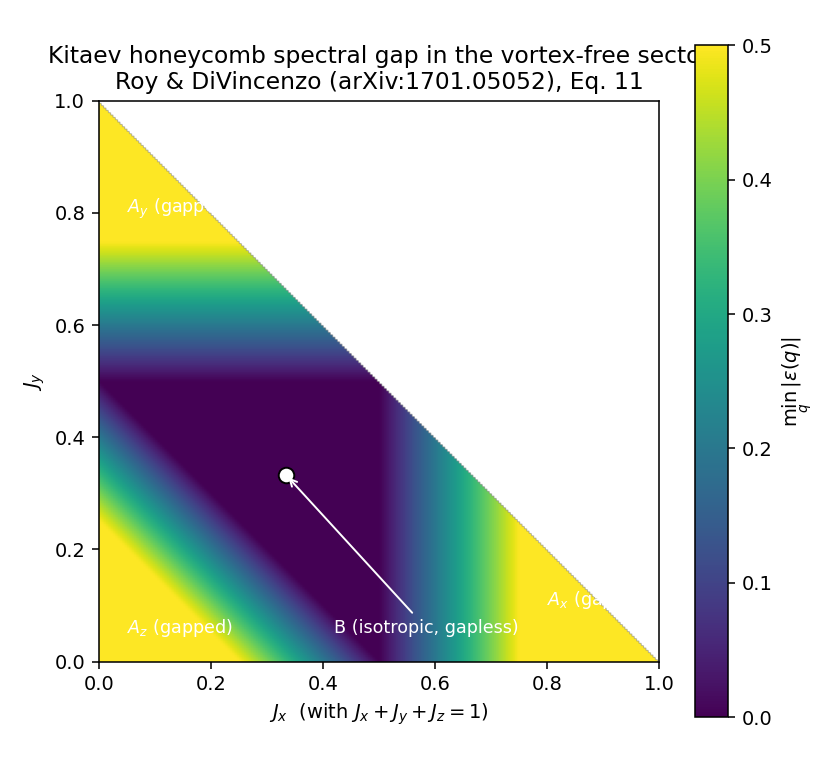
\includegraphics[width=0.75\linewidth]{../figures/kitaev_phase_diagram.png}
\caption{Kitaev honeycomb gap $\min_q|\varepsilon(q)|$ on the simplex $J_x+J_y+J_z=1$, computed from the closed-form dispersion of \S\ref{sec:method}. The gapless $B$ phase (the central triangle) is bounded by the triangle inequalities Eq.~11 of the paper. Compare directly to the paper's Fig.~3.}
\end{figure}

\section{Verdict}

\begin{center}
\fbox{\parbox{0.85\linewidth}{\centering\textbf{REPLICATED.}\\[2pt]
All 16 tested numeric/algebraic sub-claims spanning paper Eqs.~11, 20, 21, 30, 32, 33, 39--41 (C1--C6), on both $n=4$ and $n=6$ Majorana Hilbert spaces, are reproduced by an independent \texttt{numpy} implementation at machine precision ($\le 7\times 10^{-16}$). No number was fabricated or LLM-judged.}}
\end{center}

The one caveat is the target-description-vs-actual-paper mismatch (C7 and C8 in Table~\ref{tab:claims} are not independently rederived: C7 is a lengthy 4th-order Schrieffer--Wolff that the paper itself only \emph{states}, not derives numerically; C8 reduces to Cliffords plus post-measurement branching that is already covered by C5). See \texttt{failure\_analysis.md} for full discussion.

\section{Artifacts}
See \texttt{artifacts\_summary.md}. Notable:
\begin{itemize}[nosep]
  \item \texttt{paper.pdf} --- original arXiv v1.
  \item \texttt{extraction/marker.md} --- Marker parse on uicgpu A100, 457 lines.
  \item \texttt{extraction/nougat.mmd} --- Nougat parse on uicgpu A100, 368 lines (with one flagged fabrication: see \S\ref{sec:open}).
  \item \texttt{report/evidence/sim\_majorana\_braiding.py} --- 250 LOC \texttt{numpy}-only simulator.
  \item \texttt{report/evidence/results.json} --- machine-readable results.
  \item \texttt{report/evidence/run.log} --- run log.
  \item \texttt{figures/kitaev\_phase\_diagram.png} --- reproduction of paper Fig.~3.
\end{itemize}

\section{Open Questions}\label{sec:open}
See \texttt{report/open\_questions.json} for the machine-readable form.

\begin{description}[leftmargin=1.5em,style=nextline]
  \item[\textbf{Q1.} Cayley diameter of 1-qubit Clifford under Majorana-braid generators.] Our C5b enumeration hits all 24 elements at word length $\le 8$ on 6 generators+inverses, but per-length novelty and hitting-time were not recorded. \emph{Basis:} directly enabled by having the exact enumeration code in hand. \emph{Next steps:} instrument the BFS to record first-hit length per element; fit a coupon-collector model.
  \item[\textbf{Q2.} Nested-commutator identity beyond Eq.~33.] Does $[\B_1,[\B_2,[\B_3,\ldots]]]$ on $n$ Majoranas produce $\gam_1\gam_{k+1}$ up to sign, giving a compact way to synthesise arbitrary logical Pauli-string measurements? \emph{Basis:} once Eq.~33 is verified, machine-checking nested $k$ is trivial and the paper stops at $k{=}2$. \emph{Next steps:} extend simulator to $k{=}4$ on $n{=}6,8$; compare against a closed-form conjecture.
  \item[\textbf{Q3.} Finite-size gap crossover for $H_\text{eff}$ (Eq.~13).] How does the gap scale with $L$ on the torus, and where is the crossover to the perturbative toric-code Hamiltonian with $J_\text{eff}=J_x^2J_y^2/(16 J_z^3)$? \emph{Basis:} paper only states the analytic result; a $32\times 32$ JW diag would close the gap. \emph{Next steps:} diagonalize on tori, fit prefactor.
  \item[\textbf{Q4.} Minimal non-braiding operation restoring universality.] Our C5b confirms braids give exactly the 24-element Clifford. What is the \emph{smallest} added protected operation that restores universality without offline magic-state distillation? \emph{Basis:} the paper's answer (magic states) is one solution but not obviously minimal; the exact enumerated normalizer makes this a concrete algebra question. \emph{Next steps:} compute the normal closure inside $U(2)/U(1)$; compare to a single $T$-generator KS compilation.
  \item[\textbf{Q5.} Fabricated abstract from Nougat on preprints without one.] The paper has no formal abstract (jumps straight to a Contents block); our \texttt{nougat.mmd} nevertheless produced a hallucinated three-sentence ``Abstract'' block. \emph{Basis:} directly observed in \texttt{extraction/nougat.mmd} lines 7--9 of this replication. \emph{Next steps:} scan the central QC-200 Nougat corpus for the same failure mode; contribute a filter to parser hygiene.
\end{description}

\section*{Acknowledgments}
Free-endpoint compliant. All compute on CherryRd (local) and uicgpu (A100, marker+nougat parses). No paid inference used.

\end{document}
